\section{Tuesday 18 September:  Translations}

\subsection{Introduction}

\tdplotsetmaincoords{70}{110}
\begin{tikzpicture}[scale=1,tdplot_main_coords]

%set up some coordinates 
%-----------------------
\coordinate (O) at (0,0,0);
\coordinate (p1) at (0,1,0);
\coordinate (p2) at (4,1,0);
\coordinate (p3) at (4,2,0);
\coordinate (p4) at (6,0,0);
\draw [red] (O) -- (p1) -- (p2) -- (p3) -- (p4);

\draw[thick,->] (O) -- (8,0,0) node[anchor=north east]{$x$};
\draw[thick,->] (O) -- (0,3,0) node[anchor=north west]{$y$};
\draw[thick,->] (O) -- (0,0,3) node[anchor=south]{$z$};

\foreach \i in {0,60,...,360}{
	\draw [red, dashed] (0,0,0)
		 -- (0,{1*cos(\i)},{1*sin(\i)}) 
		 -- (4,{1*cos(\i)},{1*sin(\i)}) 
		 -- (4,{2*cos(\i)},{2*sin(\i)}) 
		 -- (6,0,0); 
}

\tdplotsetrotatedcoords{60}{40}{-20}
    \coordinate (Shift) at (3,5,4);
    \tdplotsetrotatedcoordsorigin{(Shift)}
\draw [red,tdplot_rotated_coords] (0,0,0) -- (0,1,0) -- (4,1,0) -- (4,2,0) -- (6,0,0);
\draw[thick,color=blue,tdplot_rotated_coords,->] (0,0,0) --
        (2,0,0) node[anchor=north]{$x'$};
    \draw[thick,color=blue,tdplot_rotated_coords,->] (0,0,0) --
        (0,2,0) node[anchor=west]{$y'$};
    \draw[thick,color=blue,tdplot_rotated_coords,->] (0,0,0) --
        (0,0,2) node[anchor=south]{$z'$};
        
\foreach \i in {0,90,...,360}{
	\draw [red, dashed,tdplot_rotated_coords] (0,0,0)
		 -- (0,{1*cos(\i)},{1*sin(\i)}) 
		 -- (4,{1*cos(\i)},{1*sin(\i)}) 
		 -- (4,{2*cos(\i)},{2*sin(\i)}) 
		 -- (6,0,0); 
}

\path (6,2,-2) node {$\{W\}$ World, global coordinate system, global frame};
\path (6,6,-2.5) node [blue] {$\{L\}$ Local coordinate system, Local frame};

\end{tikzpicture}

$\displaystyle ^{W}_{L}M$ is the matrix transformation ``$\{L\}$ with respect to $\{W\}$'', or just ``$\{L\}$ to $\{W\}$.''  

\qquad is a description of $\{L\}$ with respect to $\{W\}$.

\qquad is a matrix that converts a point in $\{L\}$ to a point in $\{W\}$.

\qquad \qquad $\displaystyle ^{W}P = ^W_LM ^LP$

\qquad is an operation that moves an object.  

\

\subsection{Conventions}

Right-handed frames (coordinate systems)

Points written as column vectors.  If row vectors, the matrices have to be transposed and the order of multiplication reversed.  

\

{\bf Transformations}  Translation, Rotation, and Scale

\subsection{Translation: Change in Position}

$P' = P + T$
\qquad
$\displaystyle 
\left[
\begin{array}{c}
	x' \cr
	y' \cr
	z' \cr
\end{array}
\right] 
=
\left[
\begin{array}{c}
	x \cr
	y \cr
	z \cr	
\end{array}
\right] 
+
\left[
\begin{array}{c}
	t_x \cr
	t_y \cr
	t_z \cr	
\end{array}
\right] 
$

\tdplotsetmaincoords{70}{110}
\begin{tikzpicture}[scale=1,tdplot_main_coords]

%set up some coordinates 
%-----------------------
\coordinate (O) at (0,0,0);
\coordinate (p1) at (0,1,0);
\coordinate (p2) at (4,1,0);
\coordinate (p3) at (4,2,0);
\coordinate (p4) at (6,0,0);
\draw [red] (O) -- (p1) -- (p2) -- (p3) -- (p4);

\draw[thick,->] (O) -- (8,0,0) node[anchor=north east]{$x$};
\draw[thick,->] (O) -- (0,3,0) node[anchor=north west]{$y$};
\draw[thick,->] (O) -- (0,0,3) node[anchor=south]{$z$};

\tdplotsetrotatedcoords{0}{0}{0}
    \coordinate (Shift) at (3,5,4);
    \tdplotsetrotatedcoordsorigin{(Shift)}
\draw [red,tdplot_rotated_coords] (0,0,0) -- (0,1,0) -- (4,1,0) -- (4,2,0) -- (6,0,0);
\draw[thick,color=blue,tdplot_rotated_coords,->] (0,0,0) --
        (2,0,0) node[anchor=north]{$x'$};
    \draw[thick,color=blue,tdplot_rotated_coords,->] (0,0,0) --
        (0,2,0) node[anchor=west]{$y'$};
    \draw[thick,color=blue,tdplot_rotated_coords,->] (0,0,0) --
        (0,0,2) node[anchor=south]{$z'$};
        

\end{tikzpicture}

\

Apply transform to every point in the mesh.  

\

OpenGL note:  Pass $M$ to the graphics system.  $M$ is applied to the vertex shader.  

We will get a {\it vertex shader}, but we will have to load it in the graphics card.  

\

\subsection{Scale:  Change in size}

$\displaystyle P' = SP
\qquad
\left[
\begin{array}{c}
	x' \cr
	y' \cr
	z' \cr
\end{array}
\right] 
= 
\left[
\begin{array}{ccc}
	s_x & 0 & 0 \cr
	0 & s_y & 0 \cr
	0 & 0 & s_z \cr	
\end{array}
\right] 
\left[
\begin{array}{c}
	x \cr
	y \cr
	z \cr	
\end{array}
\right] 
=
\left[
\begin{array}{c}
	s_x x \cr
	s_y y \cr
	s_z z \cr	
\end{array}
\right] 
$

\

In {\it uniform scale}, the three scale factors are the same.  

\vskip -1in
\tdplotsetmaincoords{70}{110}
\hfill\begin{tikzpicture}[scale=1,tdplot_main_coords]

%set up some coordinates 
%-----------------------
\coordinate (O) at (0,0,0);
\coordinate (p1) at (0,1,0);
\coordinate (p2) at (4,1,0);
\coordinate (p3) at (4,2,0);
\coordinate (p4) at (6,0,0);
\draw [red] (O) -- (p1) -- (p2) -- (p3) -- (p4);
\draw [red, dashed] (O) -- ($1.2*(p1)$) -- ($1.2*(p2)$) -- ($1.2*(p3)$) -- ($1.2*(p4)$);

\draw[thick,->] (O) -- (8,0,0) node[anchor=north east]{$x$};
\draw[thick,->] (O) -- (0,3,0) node[anchor=north west]{$y$};
\draw[thick,->] (O) -- (0,0,3) node[anchor=south]{$z$};


\end{tikzpicture}

\subsection{Rotation:  Change in Orientation}

Later in the class we'll talk more about rotation.

Example:  Rotation of $\theta$ about the $z$-axis. 

\qquad Values of $z$ do not change. 

\

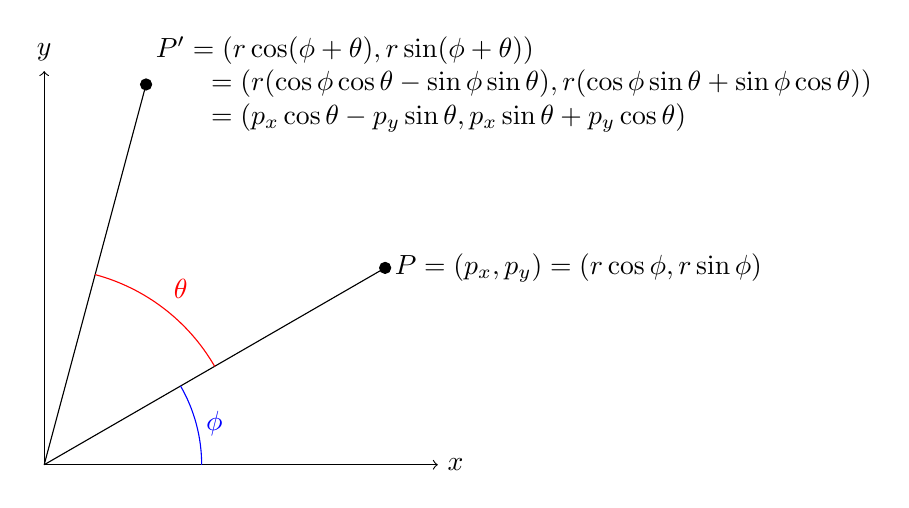
\begin{tikzpicture}[x=50mm, y=50mm]
	\draw [->] (0,0) -- (0,1) node [above] {$y$};
	\draw [->] (0,0) -- (1,0) node [right] {$x$};
	\filldraw (0,0) -- ({cos(30)},{sin(30)}) circle (2pt) node [right] {$P = (p_x, p_y) = (r \cos \phi, r\sin\phi)$};
	\filldraw (0,0) -- ({cos(75)},{sin(75)}) circle (2pt) node [right, align=left] {$P' = (r \cos (\phi + \theta),r\sin(\phi+\theta))$ 
	\\ \qquad  $= (r(\cos \phi \cos \theta - \sin \phi \sin \theta), r(\cos \phi \sin \theta + \sin \phi \cos \theta))$
	\\ \qquad  $= (p_x \cos \theta - p_y \sin \theta, p_x \sin\theta + p_y \cos \theta)$
	};
	\draw [blue] ({0.4*cos(0)},{0.4*sin(0)}) arc (0:30:0.4) node [midway, right] {$\phi$};
	\draw [red] ({0.5*cos(30)},{0.5*sin(30)}) arc (30:75:0.5) node [midway, above right] {$\theta$};
\end{tikzpicture}

\

$\displaystyle P' = R \cdot P$
\qquad 
$\displaystyle
\left[
\begin{array}{c}
	p'_x \cr
	p'_y \cr
	p'_z \cr
\end{array}
\right] 
=
\left[
\begin{array}{ccc}
	p_x \cos \theta - p_y \sin \theta \cr
	p_x \sin \theta + p_y \cos \theta \cr
	p_z
\end{array}
\right] 
= 
\left[
\begin{array}{ccc}
	\cos \theta & -\sin\theta & 0 \cr
	\sin \theta & \cos \theta & 0 \cr
	0 & 0 & 1 \cr
\end{array}
\right] 
\left[
\begin{array}{c}
	p_x \cr
	p_y \cr
	p_z \cr	
\end{array}
\right] 
$


\tdplotsetmaincoords{70}{110}
\begin{tikzpicture}[scale=1,tdplot_main_coords]

%set up some coordinates 
%-----------------------
\coordinate (O) at (0,0,0);
\coordinate (p1) at (0,1,0);
\coordinate (p2) at (4,1,0);
\coordinate (p3) at (4,2,0);
\coordinate (p4) at (6,0,0);
\draw [red] (O) -- (p1) -- (p2) -- (p3) -- (p4);

\draw[thick,->] (O) -- (8,0,0) node[anchor=north east]{$x$};
\draw[thick,->] (O) -- (0,3,0) node[anchor=north west]{$y$};
\draw[thick,->] (O) -- (0,0,3) node[anchor=south]{$z$};

\tdplotsetrotatedcoords{0}{0}{30}
    \coordinate (Shift) at (0,0,0);
    \tdplotsetrotatedcoordsorigin{(Shift)}
\draw [blue, dashed ,tdplot_rotated_coords] (0,0,0) -- (0,1,0) -- (4,1,0) -- (4,2,0) -- (6,0,0);
\draw[thick,color=blue,tdplot_rotated_coords,->] (0,0,0) --
        (2,0,0) node[anchor=north]{$x'$};
    \draw[thick,color=blue,tdplot_rotated_coords,->] (0,0,0) --
        (0,2,0) node[anchor=west]{$y'$};
    \draw[thick,color=blue,tdplot_rotated_coords,->] (0,0,0) --
        (0,0,2) node[anchor=south]{$z'$};
        

\end{tikzpicture}

\subsection{Homogeneous Coordinates and Transforms}

Add $w$ coordinate.  For now, $w=1$.
\qquad 
$\displaystyle
\left[
\begin{array}{c}
	x \cr
	y \cr
	z \cr 
	w \cr	
\end{array}
\right] 
$
represents 
$\displaystyle
\left[
\begin{array}{c}
	x/w \cr
	y/w \cr
	z/w \cr 
\end{array}
\right] 
$

\

Dividing by $w$ is called {\it homogenizing the coordinate}.

\subsubsection{Translation}

$\displaystyle
P' = T\cdot P
\qquad
\left[
\begin{array}{c}
	p'_x \cr
	p'_y \cr
	p'_z \cr
	p'_w \cr	
\end{array}
\right] 
= 
\left[
\begin{array}{cccc}
	1 & 0 & 0 & t_x \cr
	0 & 1 & 0 & t_y \cr
	0 & 0 & 1 & t_z \cr
	0 & 0 & 0 & 1 \cr
\end{array}
\right] 
\left[
\begin{array}{c}
	p_x \cr
	p_y \cr
	p_z \cr
	p_w \cr	
\end{array}
\right] 
=
\left[
\begin{array}{c}
	p_x + t_x \cr
	p_y + t_y \cr
	p_z + t_z \cr
	p_w \cr	
\end{array}
\right] 
$

\vskip 24pt

Inverse of $T$, 
$\displaystyle
T^{-1} = 
\left[
\begin{array}{cccc}
	1 & 0 & 0 & -t_x \cr
	0 & 1 & 0 & -t_y \cr
	0 & 0 & 0 & -t_z \cr
	0 & 0 & 0 & 1 \cr
\end{array}
\right] 
$

\subsubsection{Rotation of $\theta$ about the $z$-axis}

$\displaystyle
R = \left[
\begin{array}{cccc}
	\cos \theta & -\sin \theta & 0 & 0 \cr
	\sin \theta & \cos \theta & 0 & 0 \cr
	0 & 0 & 1 & 0 \cr
	0 & 0 & 0 & 1 \cr
\end{array}
\right] 
$

\vskip 24pt


$\displaystyle
R^{-1} = \left[
\begin{array}{cccc}
	\cos (-\theta) & -\sin (-\theta) & 0 & 0 \cr
	\sin (-\theta) & \cos (-\theta) & 0 & 0 \cr
	0 & 0 & 1 & 0 \cr
	0 & 0 & 0 & 1 \cr
\end{array}
\right] 
= 
\left[
\begin{array}{cccc}
	\cos \theta & \sin \theta & 0 & 0 \cr
	-\sin \theta & \cos \theta & 0 & 0 \cr
	0 & 0 & 1 & 0 \cr
	0 & 0 & 0 & 1 \cr
\end{array}
\right] 
= R^T
$

\subsubsection{Scale}

$\displaystyle
S = 
\left[
\begin{array}{cccc}
	s_x & 0 & 0 & 0 \cr
	0 & s_y & 0 & 0 \cr
	0 & 0 &  s_z &	0 \cr
	0 & 0 & 0 & 1 \cr
\end{array}
\right] 
$
\qquad
$\displaystyle
S^{-1} = 
\left[
\begin{array}{cccc}
	1/s_x & 0 & 0 & 0 \cr
	0 & 1/s_y & 0 & 0 \cr
	0 & 0 &  1/s_z &	0 \cr
	0 & 0 & 0 & 1 \cr	
\end{array}
\right] 
$
\quad (for nonzero scaling factors)

\subsection{World v/s Local Translations}

\tdplotsetmaincoords{70}{110}
\begin{tikzpicture}[scale=1,tdplot_main_coords]

%set up some coordinates 
%-----------------------
\coordinate (O) at (0,0,0);
\coordinate (p1) at (0,1,0);
\coordinate (p2) at (4,1,0);
\coordinate (p3) at (4,2,0);
\coordinate (p4) at (6,0,0);
\draw [red] (O) -- (p1) -- (p2) -- (p3) -- (p4);

\draw[thick,->] (O) -- (8,0,0) node[anchor=north east]{$x$};
\draw[thick,->] (O) -- (0,3,0) node[anchor=north west]{$y$};
\draw[thick,->] (O) -- (0,0,3) node[anchor=south]{$z$};

\tdplotsetrotatedcoords{0}{0}{30}
    \coordinate (Shift) at (0,0,0);
    \tdplotsetrotatedcoordsorigin{(Shift)}
\draw [blue, tdplot_rotated_coords] (0,0,0) -- (0,1,0) -- (4,1,0) -- (4,2,0) -- (6,0,0);
\draw [violet, tdplot_rotated_coords] (7,0,0) -- (7,1,0) -- (11,1,0) -- (11,2,0) -- (13,0,0);
\draw[thick,color=blue,tdplot_rotated_coords,->] (0,0,0) --
        (2,0,0) node[anchor=north]{$x'$};
    \draw[thick,color=blue,tdplot_rotated_coords,->] (0,0,0) --
        (0,2,0) node[anchor=west]{$y'$};
    \draw[thick,color=blue,tdplot_rotated_coords,->] (0,0,0) --
        (0,0,2) node[anchor=south]{$z'$};
        
    \coordinate (Shift) at (3,0,0);
\tdplotsetrotatedcoords{0}{0}{30}
    \tdplotsetrotatedcoordsorigin{(Shift)}
\draw [green ,tdplot_rotated_coords] (0,0,0) -- (0,1,0) -- (4,1,0) -- (4,2,0) -- (6,0,0);

\end{tikzpicture}
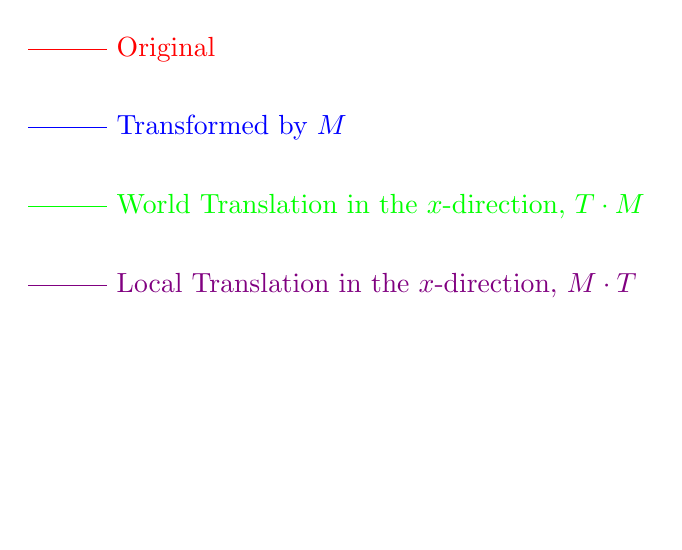
\begin{tikzpicture}
	\draw [red] (0,0) -- (1,0) node [right] {Original};
	\draw [blue] (0,-1) -- (1,-1) node [right] {Transformed by $M$};
	\draw [green] (0,-2) -- (1,-2) node [right] {World Translation in the $x$-direction, $T \cdot M$};
	\draw [violet] (0,-3) -- (1,-3) node [right] {Local Translation in the $x$-direction, $M \cdot T$};
	\path (0,-6) circle (0pt);
\end{tikzpicture}


%%% Useful Blocks of Code
\begin{comment}
$\displaystyle
\left[
\begin{array}{cccc}
	
\end{array}
\right] 
$
\end{comment}












